\documentclass[11pt]{article}

\usepackage[utf8]{inputenc}
\usepackage[english]{babel}

\usepackage{mathtools}

\usepackage{setspace}
\onehalfspacing

\usepackage{amsfonts}
\usepackage{amsmath}
\usepackage{amsthm}
\usepackage{indentfirst}
\newtheorem{theorem}{Theorem}
\newtheorem{lemma}{Lemma}
\newtheorem{example}{Example}
\newtheorem{definition}{Definition}
\newtheorem{remark}{Remark}
\newtheorem{corollary}{Corollary}

\newtheorem*{theorem*}{Theorem}
\newtheorem*{lemma*}{Lemma}
\newtheorem*{example*}{Example}
\newtheorem*{definition*}{Definition}
\newtheorem*{remark*}{Remark}
\newtheorem*{corollary*}{Corollary}

%\usepackage{booktabs, caption, graphicx, float}
%\usepackage{subcaption}
%\captionsetup{tableposition=top,figureposition=bottom,font=small}

\usepackage{comment}
\usepackage{multirow}
\usepackage{array}

\newcolumntype{C}[1]{>{\centering\let\newline\\\arraybackslash\hspace{0pt}}m{#1}}
\DeclarePairedDelimiter\floor{\lfloor}{\rfloor}

\usepackage[hidelinks]{hyperref}

\usepackage{geometry}
\geometry{a4paper, top=3cm,bottom=3cm,left=3cm,right=3cm,%
	heightrounded}
\usepackage{upgreek}
\usepackage{xparse}
\usepackage{listings}
\NewDocumentCommand{\codeword}{v}{%
	\texttt{\textcolor{black}{#1}}%
}

\newcommand{\prepos}[3]{${}_{\mathbf{#2}}{\mathbf{#1}}_{#3}$}
\newcommand{\preposm}[3]{{}_{\mathbf{#2}}{\mathbf{#1}}_{#3}}


%Dummy text
\usepackage{lipsum}

%Changing headers and footers
\usepackage{fancyhdr}
\pagestyle{fancy}
\fancyhf{}
\rhead{\textit{\thepage}}
\lhead{\textit{ Task Space Motion Control Lab}}

%For inserting the code
\usepackage{fancyvrb}

%For bold math symbols
\usepackage{bm}

%For multicolumns
\usepackage{multicol}

% Norm and abs delimiter
\usepackage{mathtools}
\DeclarePairedDelimiter{\abs}{\lvert}{\rvert}
\DeclarePairedDelimiterX{\norm}[1]{\lVert}{\rVert}{#1}

\setcounter{section}{-1}

% Argmin/Argmax
\DeclareMathOperator*{\argmax}{argmax}
\DeclareMathOperator*{\argmin}{argmin}

% Enumerate
\usepackage{enumitem}

% Code
\usepackage{algorithm}
\usepackage[noend]{algpseudocode}
\usepackage{etoolbox}

% Longtable
\usepackage{longtable}

% SI units
\usepackage{siunitx}
\sisetup{output-exponent-marker=\ensuremath{\mathrm{e}}}

% Colours in equations
\usepackage{xcolor}

\newcommand{\Rnum}{\mathbb{R}} % Symbol fo the real numbers set
\newcommand{\mat}[1]{\ensuremath{\begin{bmatrix}#1\end{bmatrix}}}	% matrix
\newcommand{\myparagraph}[1]{\paragraph{#1}\mbox{}\\}


\title{LAB 3: Task Space Motion Control}
\author{Michele Focchi and Matteo Saveriano}
\date{}

\begin{document}
	\maketitle
	\noindent
	The goals of this assignment are:
	\begin{itemize}
		\item learning the basic procedure to design a motion controller in the \textit{task} space for a manipulator in free-motion (i.e. not in contact)
		\item analyze the advantage/disadvantage of decentralized/ centralized approaches (i.e. feedback linearization)
		\item implement the control of the orientation using angle-axis representation
		%TODO \item implement the control of interaction with impedance control  
	\end{itemize}
	
	\noindent
	Tools that we are going to be using in this lab (all open-source):
	\begin{itemize}
		\item Python programming (2.7/3.5)\footnote{https://docs.python.org/}
		\item Robot Operating System (ROS)\footnote{https://www.ros.org/}
		\item Pinocchio Library for Rigid Body Dynamics Algorithms\footnote{https://github.com/stack-of-tasks/pinocchio}
		\item Locosim\footnote{https://github.com/mfocchi/locosim}
	\end{itemize}
	%
	%
	%\noindent
	In this assignment we will design a reference trajectory and close the loop at the end-effector point. 
	Then, we will design several control laws with increasing complexity, 
	evaluating their impact on the accuracy and the tracking error at the joints.
	We will learn how to deal with dynamic 
	couplings and how to appropriately solve the indeterminacy, in the case that the  
	robot is redundant with respect to the task dimension. 
	
\section{Preliminaries}
Remember to pull and recompile the framework after any update:

\begin{verbatim}
cd ~/ros_ws/src/locosim
git pull origin develop 
git submodule update
cd ~/ros_ws
catkin_make install
\end{verbatim}

%If you use Spyder use this configuration (Fig. \ref{fig:spyder}) in \codeword{Run/Configure...} to enable the interactive shell:
%
%\begin{figure}[bht]
%	\centering
%	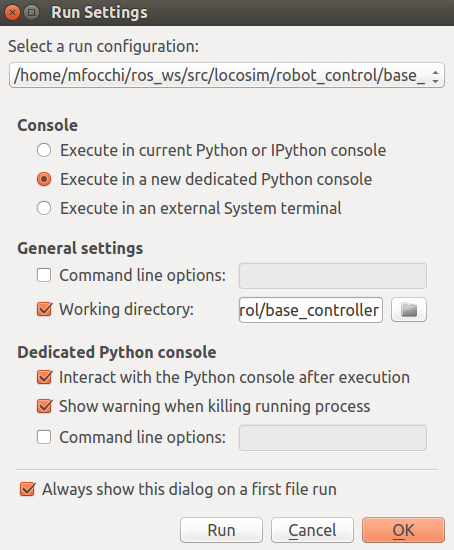
\includegraphics[width=8cm]{spyderConfig.png}
%	\caption{Spyder configuration for interactive shell.}
%	\label{fig:spyder}
%\end{figure}
%
%It is also useful to install \codeword{rope} package to enjoy auto-completion of variables with \codeword{pip install rope}.

To test the RVIZ visualization and have a grasp on the kinematic of the UR5 robot, try to move the joints with the sliders, running:
%
\begin{verbatim}
roslaunch ros_impedance_controller visualize.launch robot_name:=ur5 test_joints:=true 
\end{verbatim}

\section{Decentralized task space control (Lecture H0)}


\textbf{1.1 - Generate Sinusoidal Reference:}
Generate a sinusoidal reference for the $X$ direction of the end effector with 0.1 $m$  amplitude and 1.5 $Hz$ frequency, starting from the initial configuration $p_0 \in \Rnum^3$. 
To getn $p_0$ you need to compute the direct kinematics from $q_0$. Keep the other directions $Y$ and $Z$ at rest at 0. After 4.0 $s$ stop the sine and give a constant reference during 1.0 $s$. Note that you need to generate also consistent references for velocity and acceleration.\\



\textbf{1.2 - Step Reference generation:}
Generate a 0.1 $m$  step reference at $t= 2.0s$ for  for the $Z$ direction
 (keep the other directions with 0 reference), starting from the initial configurations $p_0$.\\


\textbf{1.3 - Inverse kinematics approach (Optional):}  Implement the end-effector tracking using inverse kinematics implemented in L1 lab, to map the end-effector position to joint space and the other differential mappings for velocity and acceleration, i.e.:


\begin{equation*}
\begin{cases}
q^d = IK(p^d) \\
\dot{q}^d =  J^{\#} \dot{p}^d \\
\ddot{q}^d =  J^{\#} ( \ddot{p}^d - \dot{J}\dot{q} )
\end{cases}
\end{equation*}

Notice that since the task is three-dimensional the Jacobian will not be square and you need to employ $J^{\#}$ rather $J^{-1}$.
Use a standard PD control to close the loop at the joint level, with a feed-forward term. Evaluate the tracking of the end-effector.\\
%Algorithm for IK: \href{https://gepettoweb.laas.fr/doc/stack-of-tasks/pinocchio/master/doxygen-html/md_doc_b-examples_i-inverse-kinematics.html}{pinocchio example}).



\textbf{1.4  Cartesian Space PD control:}
Implement a PD control law for the \textit{position} of the end-effector (that's why the word Cartesian). 


\begin{align}
\tau_c & = J^T\left(K_x(p^d - p) + D_x(\dot{p}^d -\dot{p})\right)
\end{align}

Since we are considering only the position of the end-effector you should use only the first 3 rows of the Jacobian $J \in \Rnum^{6 \times 6}$. 
Use  as  a proportional gain the positive definite matrix $K_x = 1000I_{3\times3}$ $N/m$ and as the derivative gain $D_x  = 300I_{3\times3}$ $Ns/m$. 
Try to simulate and observe how the robot behaves without any \textit{postural task} 
to solve the undeterminancy (we have a 3D task and 6 DoFs at the joints).
Use the sinusoidal reference generated in (1.1) as input to the system. Plot the tracking error, see that there is a big steady-state error due to gravity in the $Z$ direction but that there are also couplings that affect  the tracking in the 
$X$, $Y$ directions. Try to change the stiffness gain $K_x$ in the $X$,$Y$ directions and see that their tracking improves. See the joints seem to be moving randomly because we have 6 DoFs with a $3D$ task (no orientation) and there is no control in the null-space. Notice that this motion affects the tracking of the end-effector. \\


\textbf{1.5 - Cartesian Space PD control - postural task:}
Add  a secondary postural task in the joint space with  gains $K_q= 50 I_{6 \times6}$,   $D_q = 10I_{6 \times6}$ to attract the joints to a default posture $q_0$ in the joint space:

\begin{align}
\tau_0& = K_q(q_0-q) - D_q\dot{q}\\
\end{align}

to add the contributions of the two  tasks use the Null-space projector $N$ of $J^{T\#}$ to ensure that the postural task does not enter in conflict with the primary end-effector task:

\begin{align}
N & = I_{6 \times 6} - J^T J^{T\#}\\
\tau& = \tau_c  + N\tau_0 =  \tau_c  + \tau_{null}
\end{align}

Observe that the joints now are no longer wobbling around, and the tracking of the end-effector is no longer affected by the random motion of the joints. 
This is because this lives in the null-space of $J^{T\#}$ (that has the same dimension of the null-space of $J$) that is the set of torques that do not affect the end-effector motion. Note that still there are steady-state tracking errors due to gravity.\\


\textbf{1.6 - Cartesian Space PD control + Gravity Compensation:}
Add a gravity compensation term computed in the task space $G= J^{T\#}g$).

\begin{align}
\tau & = J^T\left( K_x(p^d - p) + D_x(\dot{p}^d -\dot{p})  + J^{T\#}g \right) + \tau_{null}
\end{align}

Give the step reference generated in (2.1) as input to the system. 
Check there is no longer a  tracking error at steady state but  it still it is present during the transient. \\


\textbf{1.7 - Cartesian PD control  + Gravity Compensation + Feed-Forward term:}
Add also a feed-forward acceleration action to the PD control. Use the the reflected inertia
at the end-effector $\Lambda = (J M^{-1} J^T)^{-1}$ (note that we no longer use only the diagonal elements!):

\begin{align}
\tau & = J^T\left( \Lambda \ddot{p}^d + K_x(p^d - p) + D_x(\dot{p}^d -\dot{p})  + J^{T\#}g \right) + \tau_{null}
\end{align}

Note that J should be full row rank  otherwise you need to add a damping term to make $JM^{-1}J^T$ invertible.
We employ the expression of $\Lambda = (JM^{-1}J^T)^{-1}$ because this is valid also for redundant robots, while $\Lambda = J^{-T}M J^{-1}$ is only  valid for non-redundant robots. 
Give the sinusoidal reference generated in (1.1). See that the tracking error is improved for a time-varying reference on the $X$ direction, but still there are tracking errors on $Y$ and $Z$ direction due to the inertial couplings and to the non-consistency of the initial state (for velocity).\\

\section{Centralized task space control (Lecture H0)}

Similarly to what we did in the joint space case, to effectively compensate for the inertial couplings, we will compensate them by linearizing the Cartesian dynamics of the robot (i.e. reflected at the end-effector) via a state feedback.\\


\textbf{2.1 - Cartesian space inverse dynamics (computed torque):}
Implement Cartesian space inverse dynamics with a postural task in the null space of the end-effector task, to fulfill the task and at the same time attract the robot to a configuration $q_0$. 
Note that because our robot is redundant for the (3D) positioning task the Jacobian is rectangular and we will have to use the $J^{\#}$ in place of the $J^{-1}$:

\begin{align}
&F^d = \ddot{p}^d + K_x(p^d - p) + D_x(\dot{p}^d -\dot{p})  \\
& \Lambda = (J M^{-1}J^T)^{-1}\\
&\mu(q,\dot{q})  = J^{T\#} h -\Lambda \dot{J} \dot{q} \\
&\tau  = J^T\left( \Lambda F^d +  \mu(q,\dot{q}) \right) + \tau_{null}
\end{align}


Observe that the tracking is now almost perfect, there are no coupling between different directions anymore.  Observe that if you reduce the gains the tracking remains good apart in the discontinuity at the end of the sinusoidal trajectory.  \\



\textbf{2.2 - Cartesian space inverse dynamics - simplified:}
Rather than compensate for the bias terms reflected at the end-effector $\mu(q,\dot{q})$,  compensate for them at the joint space level ($h$) and observe that the result is the same. 
\begin{align}
&F^d = \ddot{p}^d + K_x(p^d - p) + D_x(\dot{p}^d -\dot{p})  \\
&\tau  = J^T\left( \Lambda F^d  \right) + h + \tau_{null}
\end{align}

The advantage of this (less elegant) approach is that it saves us the computation of the terms $\dot{J}$ and $J^{T\#}$.\\


\textbf{2.3 - External Force:}
With constant reference $x_0$,  apply an external force  $F_{ext} = \mat{0.0 & 0.0 & 200}^T N$ (i.e. on the
$Z$ direction) at t = 1 $s$ and check that, thanks to the inverse dynamics, 
only the end-effector position in the $Z$ direction is affected, but not on $X$ and $Y$. 
If you reduce by half the $K_x$ gains you should see the deflection due to $F_{ext}$ 
it doubles (because the system is linearized).


\section{Orientation control (Lecture H1)}

Until now we only defined a 3D task for the end-effector position. Now we want also to control the orientation and define a full 6D task. 
The secondary postural task will no longer be necessary because the dimension of the task is the same as the number of joints (i.e. dimension of the joint space). Note that you can control orientation employing different parametrizations of the orientation to compute the orientation error. \\


\textbf{3.1 - PD control of end-effector position + orientation:}
Now we want also to control  the orientation  of the end-effector (advice: the Jacobian is now $6\times6$ ). 
Implement a PD control law and use the \textit{angle-axis} representation to compute the orientation error ${}_we_o$. 

First define the rotation matrix that represents the desired orientation, ${}_wR_d = [\hat{x}_d, \hat{y}_d, \hat{z}_d]$ with  ($\hat{x}_d$ axis along $\hat{x}_w$, $\hat{y}_d$ axis  along $-\hat{y}_w$, $\hat{z}_d$ axis along $-\hat{z}_w$). This is equivalent to rotate the world frame 180 degrees with respect to its $X$ axis. % for some reason the result is opposite for rotations smaller that 180 degs TODO
Then compute the rotation matrix that represents the relative rotation from the \textit{actual} end-effector orientation ${}_wR_{ee}$ to the \textit{desired} orientation ${}_wR_d$:

\begin{align}
&{}_{ee}R_d = {}_wR_{ee}^T {}_wR_d
\end{align}

then, the orientation error ${}_{ee}e_o$ could be computed from the angle-axis associated to ${}_{ee}R_d$:


\begin{align}
& {}_{ee}e_o = \Delta\theta \hat{r}
\end{align}

where the unit axis $\hat{r}$  and the scalar $\Delta \theta$ could be computed from 
the relative orientation matrix ${}_{ee}R_d$ (that we name $R$ in this formula): 

\begin{align}
& \Delta \theta = acos\left(\frac{R_{1,1} + R_{2,2} +R_{3,3} -1}{2}\right)\\
&\mat{\hat{r}_x \\ \hat{r}_y\\ \hat{r}_z} = \frac{1}{2sin \delta \theta} \mat{R_{3,2} - R_{2,3} \\R_{1,3} - R_{3,1}\\R_{2,1} - R_{1,2}}
\end{align}



Note that  the orientation error ${}_{ee}e_o$ it is expressed in the end-effector frame,
we need to map it in the world frame to compute the moment because the jacobian $J$ is expressed in the WF:

\begin{align}
&e_o = {}_wR_{ee} ~{}_{ee} e_o
\end{align}

We can extract the angular velocity of the end-effector frame as the angular part of the 6D \textit{twist} obtained as:

\begin{equation}
\mat{\dot{p}\\ \omega} = J_{6\times6} \dot{q}
\end{equation}

Now, we can write the PD law using the orientation proportional $K_{o} = 800I_{3\times3}$ and damping $D_o = 30I_{3\times3}$ gains, setting the desired angular velocity to  $\omega^d = \mat{0&0&0}^T$: 

\begin{align}
& \Gamma^d  = K_{o} e_o  + D_o(\omega^d - \omega)  \\
\end{align}

Finally, we stack the orientation task $\Gamma^d$ below  the Cartesian task $F^d$ (that was previously computed) to form the desired \textit{wrench} $W^d$ that we can map to torques via $J^T$ and compensate for gravity:
\begin{align}
&W^d=\mat{F^d \\ \Gamma^d}\\
&\tau = J^TW^d + g
\end{align}

Plot   the  orientation error and see that is going to zero.
 Note that, since you used a PD control law,  you will have tracking errors (both in the linear and in the angular  coordinates) because of gravity and inertial couplings. Additionally, you will notice that increasing the damping gain  $D_o = 30I_{3\times3}$ beyond 30 makes the system unstable.
We saw that the acos(.) function provides an output only in the $\mat{ 0 , \pi}$ range. 
instead, use the atan2(.) function to compute  $\Delta \theta$, that provides output in $\mat{ -\pi   , \pi }$.\\

\begin{equation}
\Delta \theta = atan2\left(\sqrt{(R_{3,2} - R_{2,3})^2 + (R_{1,3} - R_{3,1})^2 + (R_{2,1} - R_{1,2})^2}, tr(R) -1\right)
\end{equation}






\textbf{3.2 - PD control of end-effector position + orientation - singularity:}
Now we want to change the orientation set-point  ${}_wR_{d}$ at will. To do so 
is is convenient to use Euler Angles. Define the sequence (note that it is not a vector!)  
$\Phi^d$ of Euler Angles in ZYX convention that represent the desired orientation 
and map it into ${}_wR_{d}$ using the function  \codeword{eul2Rot}($\Phi^d$). 

To check the tracking in terms of Euler Angles you need to convert the rotation matrix ${}_wR_{ee}$ 
that represents the actual orientation  into the correspondent Euler Angles using the dual function \codeword{rot2eul}(${}_wR_{ee}$).

Set some values for the sequence $\Phi^d$ such that the representation is at singularity (i.e. $\theta = \pi/2$), 
and see that while the error orientation angle-axis is still continuous, the 
plot of the Euler Angles representation suffers from discontinuities because of the singularity. 
This is one of the reasons for which we chose to close the loop on orientation error and not on Euler Angles for orientation control. \\
With angle-axis we still have a singularity for $\Delta \theta = 0$ that you can deal with explicitly returning zero orientation error in that case.\\



 

\textbf{3.3 - PD control of end-effector position + orientation - sinusoidal reference:}
Try to set a sinusoidal reference (which mimics a drilling operation)  $ 2.2 \pi sin(t)$ for the desired roll angle $\psi^d$ and 0.0 for desired pitch and yaw. Remember that you should also compute a consistent time-varying reference also for the angular velocity $\omega^{d}$ in a PD control law. In this case, remember that you need to compute the derivatives of the Euler Angles (Euler rates) and map  them into $\omega$ via  $\omega^d = T_{\omega}(\Phi^d)\dot{\Phi}^d$. Set a constant end-effector reference to better visualize the motion.
Plot the tracking for the Euler Angles.\\


\textbf{3.4 - PD control of end-effector position + orientation - unwrapping:}
Note that the roll signal switches between $\pi$ and $-\pi$ as in Fig. \ref{fig:rpy}. You do not see this in the orientation error because is always in the range $\pi$ and $-\pi$. Implement an \textit{unwrapping} algorithm to avoid this phenomena and get a continuous plot:

\begin{figure}[H]
	\centering
	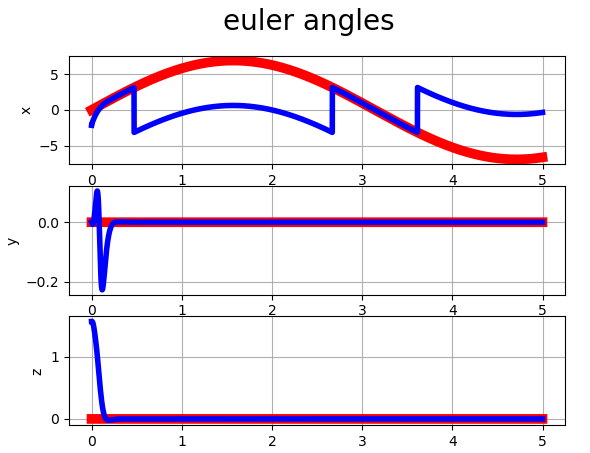
\includegraphics[width=8cm]{pics/euler_angles_tracking.png}
	\caption{Tracking of Euler Angles that suffers from the effect of wrapping.}
	\label{fig:rpy}
\end{figure}

\begin{verbatim}
for i in range(3):
    rpy_unwrapped[i] = rpy[i];
    while (rpy_unwrapped[i] < rpy_old[i]  - math.pi):
        rpy_unwrapped[i] += 2*math.pi
    while (rpy_unwrapped[i] > rpy_old[i]  + math.pi):  
        rpy_unwrapped[i] -= 2*math.pi
    rpy_old[i] = rpy_unwrapped[i] 	
\end{verbatim}

Check at the end of this \href{https://youtu.be/sax0QzG8qAw }{video} what can happen to your robot, if you do not do the unwrapping and you close the loop on Euler Angles to control orientation! \\
%Why the motion of the joints seems weird? Remember the concept dexterous workspace? Unfortunately even if in theory you could be able to specify both positions and orientations of the end-effector frame, this does not mean that you can specify any arbitrary orientation for all end-effector positions in the primary workspace (remember definition of dexterous workspace). This means that in some locations you might not be able to achieve every possible orientation, but just a subset of them. 
%A way to increase the size of the dexterous workspace and be more free to specify any orientation is to add a deegree of freedom of redundancy (e.g. use 7 DoFs robot) %"natural" motion! 


\textbf{3.5 - Control of orientation using quaternions (optional):}
Implement the computation of the orientation error with the 
quaternion representation and check that it gives the same result as closing the loop with the angle-axis representation. \\


\textbf{3.6 - Implement the full (6D) task space inverse-dynamics:}
Implement the full inverse dynamics algorithm to remove the inertial/coriolis couplings and gravity for a 6D task.
Observe that the inertia reflected at the end-effector $\Lambda$ is now a $6\times6$ matrix and should be recomputed from the $6\times6$ Jacobian. Note that this matrix 
can become singular if the Jacobian (now square) is singular. 
Actually, verify that the rank of the Jacobian drops from 6 to 5 in the initial position $q_0$ therefore some mobility is lost 
at the very beginning.

 \begin{equation}
  J = \mat{-0.19145 &0.27456& -0.08306 &-0.08306 & 0.07223 & 0. \\    
  0.5765&   0.    &   0.  &     0.   &    0.  &     0.     \\
  0.    &  -0.5765 & -0.34687&  0.04538 -0.03946  &0.     \\
  0.  &     0.  &     0.    &   0. &     -0.47943 & 0.     \\
  0.  &     1.  &     1.    &   1.  &     0.      & 1.     \\
  1.  &     0.  &     0.    &   0.&      -0.87758 & 0.     }
 \end{equation}

How do you solve this? Try to set a threshold $\rho = 0.0001$ for the singular values in the 
SVD decomposition in the \codeword{np.linalg.pinv} function or, equivalently, implement  a damping in the pseudo-inverse of $J^T$ as follows and check that they produce the same output: 

\begin{equation}
J^{T\#} = \left(J J^T + I_{6\times 6}\rho^2\right)^{-1}J
\end{equation} 

Remember that for this control law we need also to add the desired \textit{acceleration} terms (both linear and angular) and we are still missing the $\dot{\omega}^d$ term. $\dot{\omega}^d$ can be obtained in a similar way to the desired angular velocity, by differentiating the previous relationship:

\begin{equation}
\dot{\omega}^d = T_{\omega}(\Phi^d) \ddot{\Phi}^d +  \dot{T_{\omega}}(\Phi^d,\dot{\Phi}^d ) \dot{\Phi^d}
\end{equation}

Note that the postural task is no longer needed, because we are assigning a $6D$ task. Therefore, the full control law is:
 
\begin{align}
& F^d = \ddot{p}^d + K_x(p^d - p) + D_x(\dot{p}^d -\dot{p})  \\
& \Gamma^d  = \dot{\omega}^d + K_{o} e_o  + D_o(\omega^d - \omega)  \\
& W^d = \mat{F^d \\ \Gamma^d} \\
& \Lambda = (J M^{-1}J^T + \rho^2 I_{6 \times6})^{-1}\\
&\mu(q,\dot{q})  = J^{T\#} h -\Lambda \dot{J} \dot{q} \\
& \tau = J^T\left( \Lambda W^d + \mu \right)
\end{align} 

Verify that the tracking is almost perfect (apart from the transient due to the difference from the initial state and the reference) both during the motion and at steady-state, showing a perfect cancellation of all the non-linear terms, making the system linear and decoupled. 
An important consequence is that you can now increase at will the damping gain  $D_o = 30I_{3\times3}$ beyond 30 without making the system unstable.

%\section{Interaction control (Lecture H2)}
 
\end{document}